\subsection{Trigonometry}

\begin{enumerate}
	\item
	\begin{enumerate}[topsep=0ex,itemsep=0ex,partopsep=1ex,parsep=1ex]
		\item[(a)] Define the following terms
		\begin{enumerate}[topsep=0ex,itemsep=0ex,partopsep=1ex,parsep=1ex]
			\item[i)] Sine
			\item[ii)] Tangent
		\end{enumerate}
		
		\item[(b)] Evaluate $\tan15 \degree + \cot75 \degree$. Give the answer in simplest form.
		
		\item[(c)] Prove that $(1 - \cos{A})(1 + \cos{A}) = \sin{A}\tan{A}$
	\end{enumerate}

	\item
	\begin{enumerate}[topsep=0ex,itemsep=0ex,partopsep=1ex,parsep=1ex]
		\item[(a)] 
		\begin{enumerate}[topsep=0ex,itemsep=0ex,partopsep=1ex,parsep=1ex]
			\item[i)] Express $\sin3\theta$ in terms of $\sin\theta$
			\item[ii)] Show that $\sqrt{\frac{(1 - \cos{\phi})}{1 + \cos{\phi}}} = \csc{\phi} - \cot{\phi}$
		\end{enumerate}
		
		\item[(b)] Given the figure below,
		\vspace*{-7mm}
		\begin{center}
			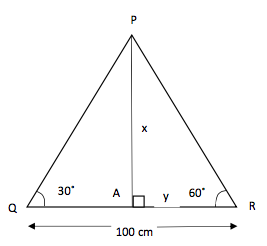
\includegraphics[width=0.45\textwidth]{./img/math_BAM_trig_1.png}
		\end{center}
		\begin{enumerate}[topsep=0ex,itemsep=0ex,partopsep=1ex,parsep=1ex]
			\item[i)] Determine the values of $x$ and $y$
			\item[ii)] Find $\sin(Q\hat{P}A)$
		\end{enumerate}
	\end{enumerate}
	
	\item
	\begin{enumerate}[topsep=0ex,itemsep=0ex,partopsep=1ex,parsep=1ex]
		\item[(a)] Without using a mathematical table or calculator, evaluate:
		\begin{enumerate}[topsep=0ex,itemsep=0ex,partopsep=1ex,parsep=1ex]
			\item[i)] $\cos(165 \degree)$
			\item[ii)] $\tan(A + B)$ given that A and B are acute angles having $\sin(A) = \frac{7}{25}$ and $\cos(B) = \frac{5}{13}$
		\end{enumerate}
		
		\item[(b)] 
		\begin{enumerate}[topsep=0ex,itemsep=0ex,partopsep=1ex,parsep=1ex]
			\item[i)] Find the values of $x$ that satisfy the equation $\sin{2x} + \cos{x} = 0$ for $0 \degree \leq x \leq 360 \degree$
			\item[ii)] Verify that the solution of the equation in part (b) i) can be obtained graphically by plotting the graph of $y= \sin{2x} + \cos{x}$ for $0 \degree \leq x \leq 360 \degree$
		\end{enumerate}
	\end{enumerate}

\end{enumerate}










